\chapter{Materials and Methods}
\label{Materials and Methods}
\paragraph{}

The product contains two main things that need to understand: making the model that is reliable enough to minimize the percentage of allowing a person that is not in the database can control the lock and making the connection between the recognition system to the \acrshort{ccu} fastest, without delay, and most secure. Face recognition plays a role as an authentication layer, allow the action will be authenticated before start. To understand face recognition, we have to study image classification and feature extraction. \acrshort{iot} connection is responsible as a bridge layer to smart devices. Making it fast and instantly is easy, but we have to research blockchain connections for securing the connection.

With the proposed problem, we have split it into more minorissues:

\begin{itemize}
    \item How can we detect faces in the camera stream.
    \item How to capture one frame containing a face from the camera stream.
    \item How to resize the captured frame from a full HD resolution to a smaller size.
    \item How can we verify the face in the captured frame.
    \item Which architecture of the model we are aiming to build.
    \item Which way to connect and control \acrshort{iot} devices.
    \item How to secure the connection between the recognition system to \acrlong{ccu}.
\end{itemize}

To solving above problem, there are some tools and libraries we need to solve it:

\begin{itemize}
    \item \textbf{OpenCV}: Using to resize the original frame to a smaller size, converting the image to grayscale for quickly detecting faces and further reducing the computational complexity. Besides, we need OpenCV to capture frames from a connected camera.
    \item \textbf{Haar Cascade}: Using for detecting faces.
    \item \textbf{\acrlong{mtcnn}}: Help us to extract keypoints of faces. With keypoints, we can measure if the presented face is a real face.
    \item \textbf{One-shot learning}: One-shot learning is used for reducing the retraining model from scratch problem when there is a newcomer.
\end{itemize}

To connect between the face recognition server to \acrlong{ccu} for approving access to control \acrshort{iot} devices, we are using \textbf{Flask} because of its simplicity in development and maintenance.

\section{Materials}

\subsection{OpenCV}
\paragraph{}

\begin{figure}[H]
    \centering
    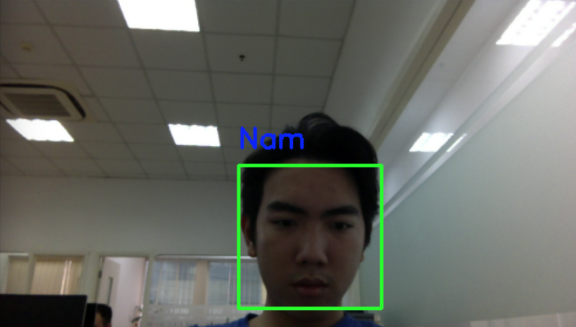
\includegraphics[scale=0.6]{opencvExmaple.png}
    \caption{OpenCV Example}
\end{figure}

OpenCV was introduced at Intel in the year 1999 by Gary Bradsky. The first release came in late 2000. OpenCV represents for Open Source Computer Vision Library. Even though it is written in optimized C/C++, it has interfaces for Python and Java alongside C++. OpenCV has an active user base worldwide, and the number of users is increasing day by day due to the rise in computer vision applications.

OpenCV uses for image and video analysis, like facial detection, license plate reading, photo editing, advanced robotic vision, optical character recognition, and many more. OpenCV-Python is the Python API for OpenCV. It acts like a python wrapper around the C++ implementation of OpenCV.

OpenCV-Python is fast, and it is not difficult to code and deploy(due to the Python wrapper in the foreground). This makes it a great choice to perform computationally intensive programs. 

\subsection{Haar Cascade}
\paragraph{}
The main aim of face recognition is to detect faces in the frame. Haar cascade is one of the fast, effective ways to achieve it. First published by Paul Viola and Michael Jones\cite{haarcascade} in 2001, it is a machine learning approach to detect almost any object, but it mainly solves face detection problems. 

\begin{figure}[H]
    \centering
    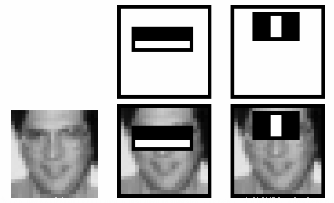
\includegraphics[scale=1.3]{haar.png}
    \caption{Haar Cascades}
    \caption*{\textit{source: docs.opencv.org}}
\end{figure}

Haar Cascade can understand using many \textbf{Haar} features and then using those features many times (\textbf{Cascade}) to build up a face detection. It has four steps: 
Haar Cascade can understand using many \textbf{Haar} features and then using those features many times (\textbf{Cascade}) to build up to face detection. It has four steps: 

\subsubsection{Haar Feature extraction}

\begin{figure}[H]
    \centering
    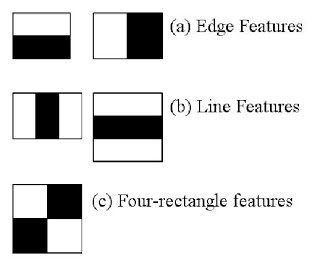
\includegraphics[scale=0.7]{haar_features.png}
    \caption{Four Haar Features}
    \caption*{\textit{source: docs.opencv.org}}
    \label{fig:haarFeature}
\end{figure}

First, we have to collect the Haar feature. As a feature to encode every domain is operate faster than pixel system, objects are mainly classified on many simple features. A \textbf{Haar Feature} is a calculation performed on adjacent rectangular regions on a specific location in the window. Haar Feature is shown in figure~\ref{fig:haarFeature} below.

\subsubsection{Integral Image Representation}
Integral Images efficiency speed up the calculation of these Haar features in one pass over the image. It creates sub-rectangles and creates array references for each sub-rectangles instead of computing at every pixel—figure~\ref{fig:integralImage} followed by Zhang, Cha, and Zhang, Zhengyou \cite{book}.

\begin{figure}[H]
    \centering
    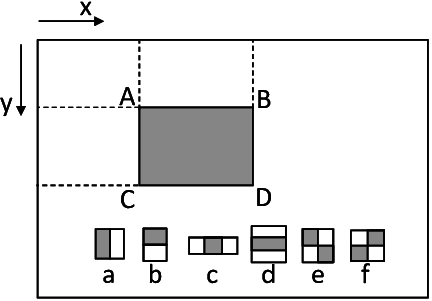
\includegraphics[scale=0.6]{integralImage.png}
    \caption{How integral image works}
    \label{fig:integralImage}
\end{figure}

\subsubsection{Adaboost Training}
As we do not know which Haar classifier is the best fit, we have a solution to group every weak classifier into a robust classifier using \textbf{Adaboost} (adaptive boosting). It chooses the best features and trains the classifier to use them. 

\begin{figure}[H]
    \centering
    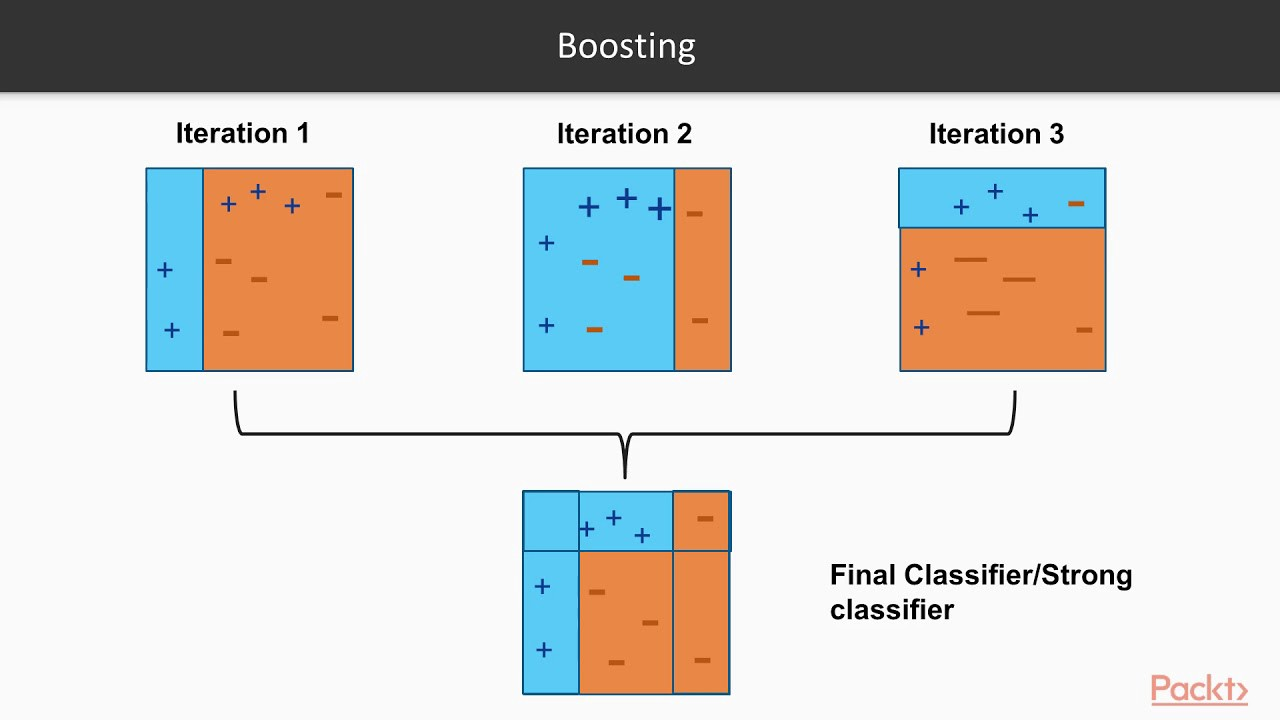
\includegraphics[scale=0.2]{adaptiveBoost.png}
    \caption{Adaptive boosting algorithm}
    \caption*{\textit{source: Packt}}
\end{figure}

\subsubsection{Cascading Classifier Architecture}
Paul Viola and Michael Jones ensured in their paper that employing a \textbf{cascade of classifiers} makes the algorithm performs faster. The cascade classifier consists of series of stages, and each stage contains a collection of strong classifiers. It removes the need to apply all features on a window simultaneously. Every time the sub-window slides into a window, if it detects the face, we move to the next step; else, we discard that region and slide to another part. The rejected region will keep at rejected sub-windows. The process is shown in diagram\ref{fig:cascadeStructure}, originally from Lee, Deok Gyu et al.\cite{article}.

\begin{figure}[H]
    \centering
    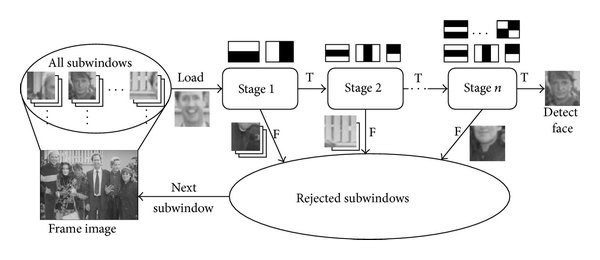
\includegraphics[scale=0.8]{cascadeStructure.jpeg}
    \caption{Cascade structure of Haar classifier}
    \label{fig:cascadeStructure}
\end{figure}

\subsection{\acrlong{mtcnn}}
\paragraph{}
\acrlong{mtcnn} (\acrshort{mtcnn}) is a solution for both face detection and face alignment. Proposed by Zhang et al.\cite{Zhang_2016}, it is one of the most popular and accurate face detection tools today. This model has three \acrlong{cnn} (P-Net, R-Net, O-Net) connected in a cascade.

\begin{figure}[H]
    \centering
    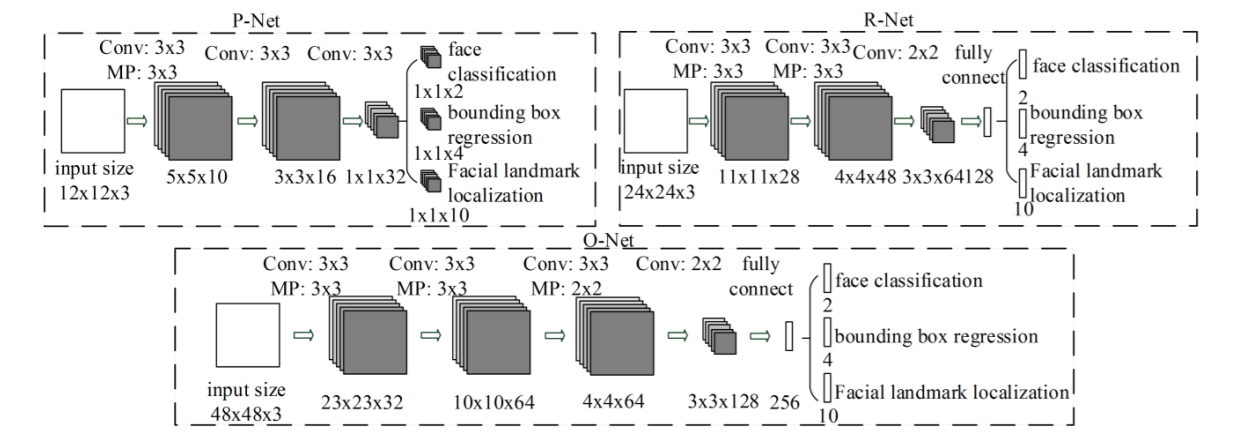
\includegraphics[scale=0.4]{mtcnnArchitecture.png}
    \caption{MTCNN structure}
\end{figure}

\acrshort{mtcnn} can integrate both recognition and alignment because of multi-task learning. There are three-stage corresponding to three \acrshort{cnn}. In the first stage, the Proposal Network (P-Net) quickly produces windows thanks to a shallow \acrshort{cnn}. The Refine Network (R-Net) refines the proposed candidate windows into a more complex \acrshort{cnn} to the second stage. Lastly, Output Network (O-Net) is more complicated than others, refining the result and showing the facial landmark positions.

\subsection{One-shot learning}
\label{oneShot}
\paragraph{}
One-shot learning is a supervised algorithm that only needs one or only a few pictures for each class. We use a simple \acrshort{cnn} algorithm to predict who it is from the input picture of one class.

\begin{figure}[H]
    \centering
    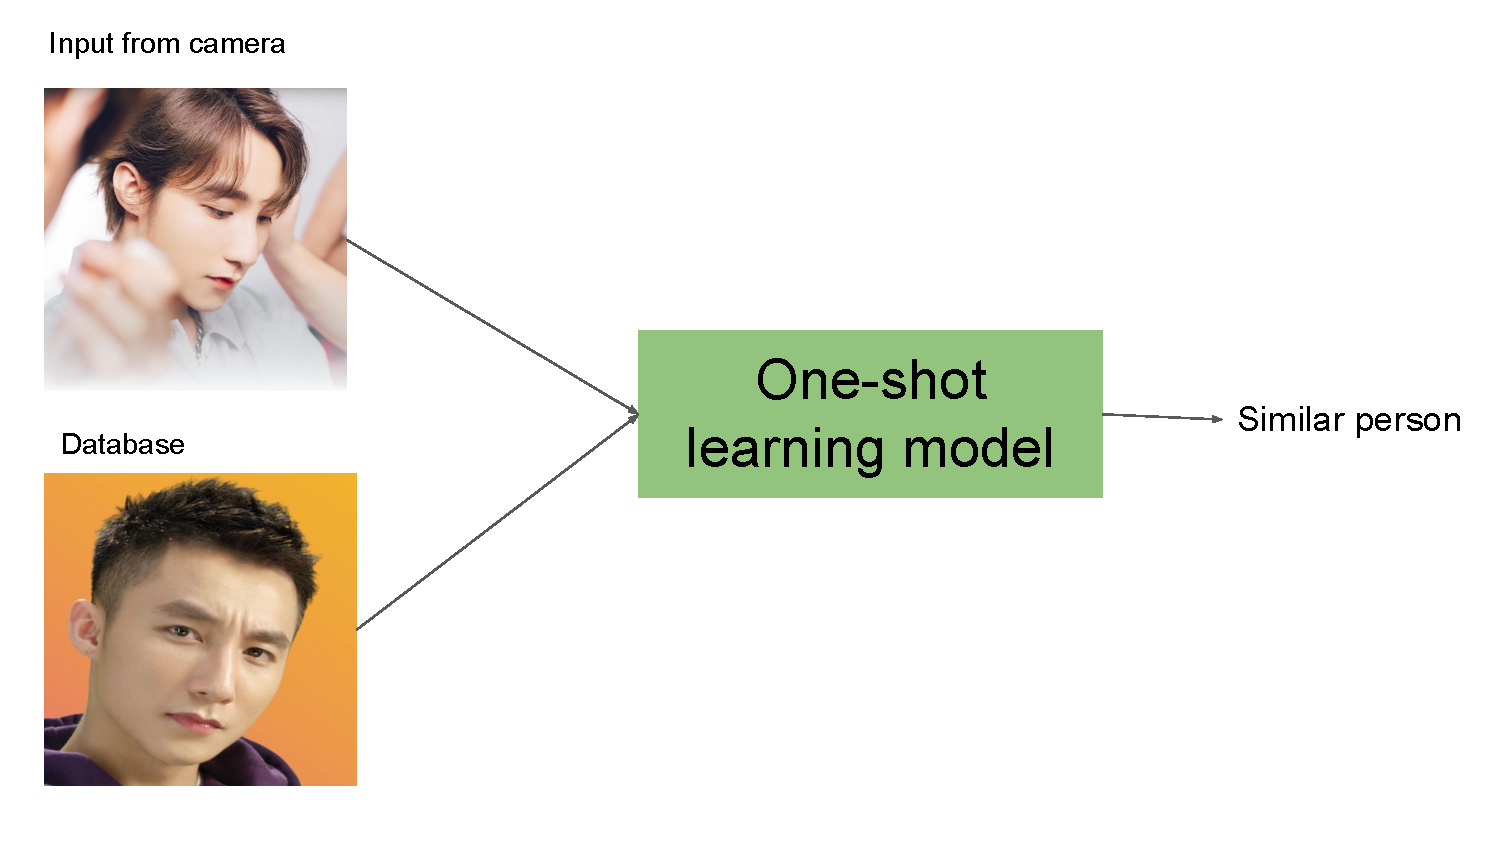
\includegraphics[scale=0.5]{oneShotLearning.pdf}
    \caption{One-shot learning example}
\end{figure}

This method will save much man’s power and power consumption. Because we only a little picture, every time newcomers show up, we will make it easier by taking only one picture of them. And the process of creating embeddings for existing images is also taking less time than the traditional way that is training a model with thousands of pictures for each class. We can scale up the system for a large number of classes quickly.

\subsection{Learning similarity}
\paragraph{}
Learning similarity is based on a distance calculation between two pictures, usually a $\ell_1$, $\ell_2$ norm so that if that is the same person, the distance will be smallest, else it will be biggest:

\begin{center}
    $
    \begin{cases}
    d(img1,img2) \leq \tau \Rightarrow \text{same}\\
    d(img1,img2) \geq \tau \Rightarrow \text{different}\\
    \end{cases}
    $
\end{center}

When using this method, we have to choose a threshold to decide if this picture is the same or different. For example, in figure~\ref{fig:learnSimilar}, if the image from the left has a distance smaller than the threshold, which is 0.2, then it is the same picture:

\begin{figure}[H]
    \centering
    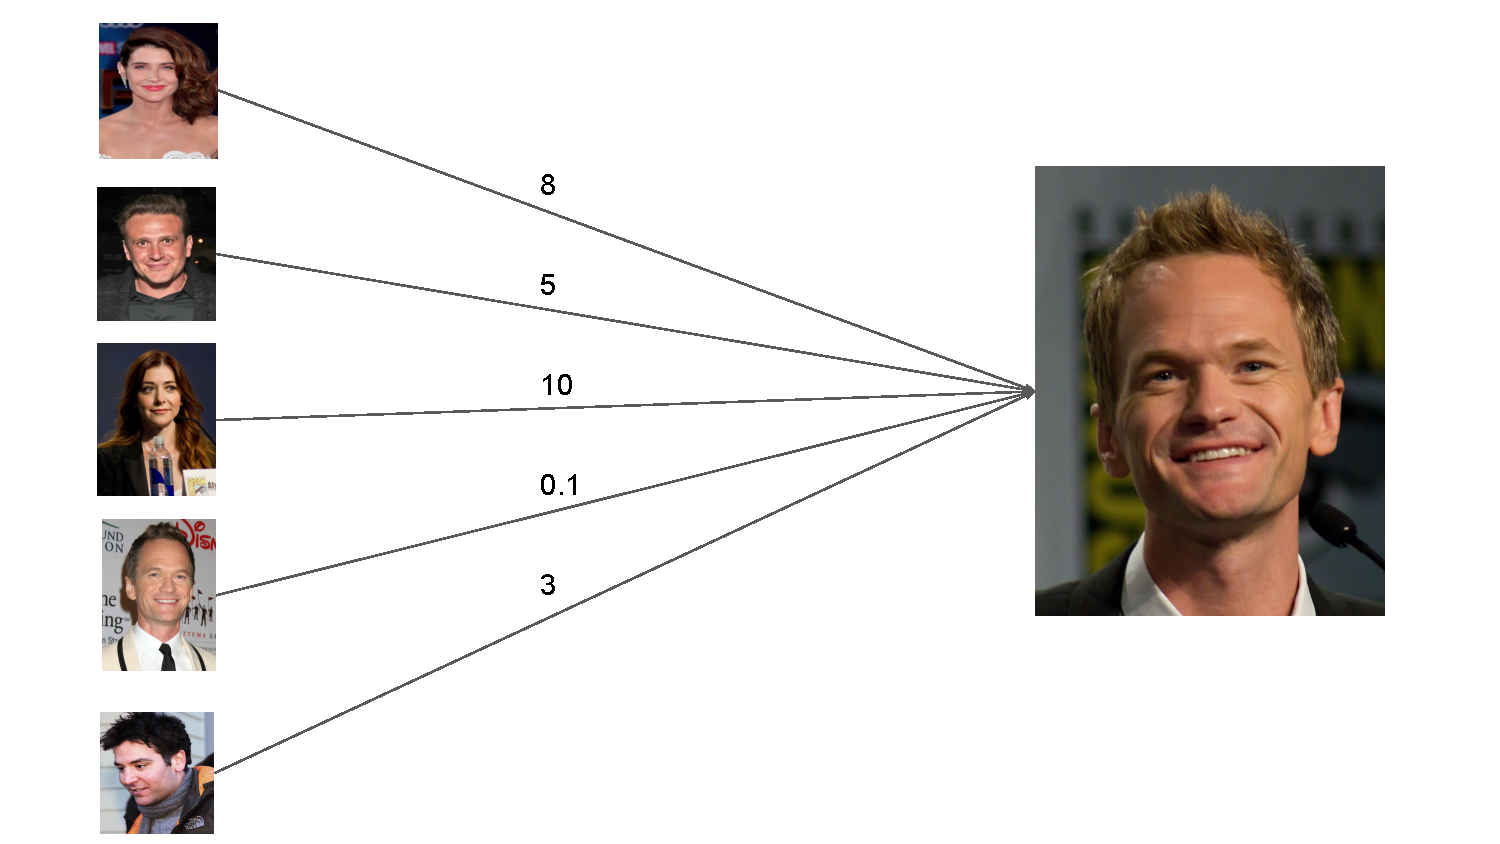
\includegraphics[scale=0.5]{learningSimilarity.pdf}
    \caption{Learning similarity method}
    \label{fig:learnSimilar}
\end{figure}

We can see that learning similarity has the advantage that we can find the similarity picture without re-training the model again. Besides, it will not depend on the number of classes. So we do not have to train the model again when there is a new class. 

\subsection{Siamese neural network}
\label{sec:siamese}
\paragraph{}
Siamese network was first introduced by Yaniv Taigman et al.\cite{inproceedings}. It is a network architecture that can answer if two pictures are the same person in it. The architecture of a Siamese network is a \acrlong{cnn} without an \textbf{output layer} to encoding a picture to an embedding vector. The input of a Siamese network is two random pictures chosen from the database. After the network handling it, it returns two vectors corresponding to two input pictures. The \textbf{loss function} is responsible for calculating the distance between two vectors to show the difference between them. Usually, the loss function in this network is a $\ell^2$-norm function.

\begin{figure}[H]
    \centering
    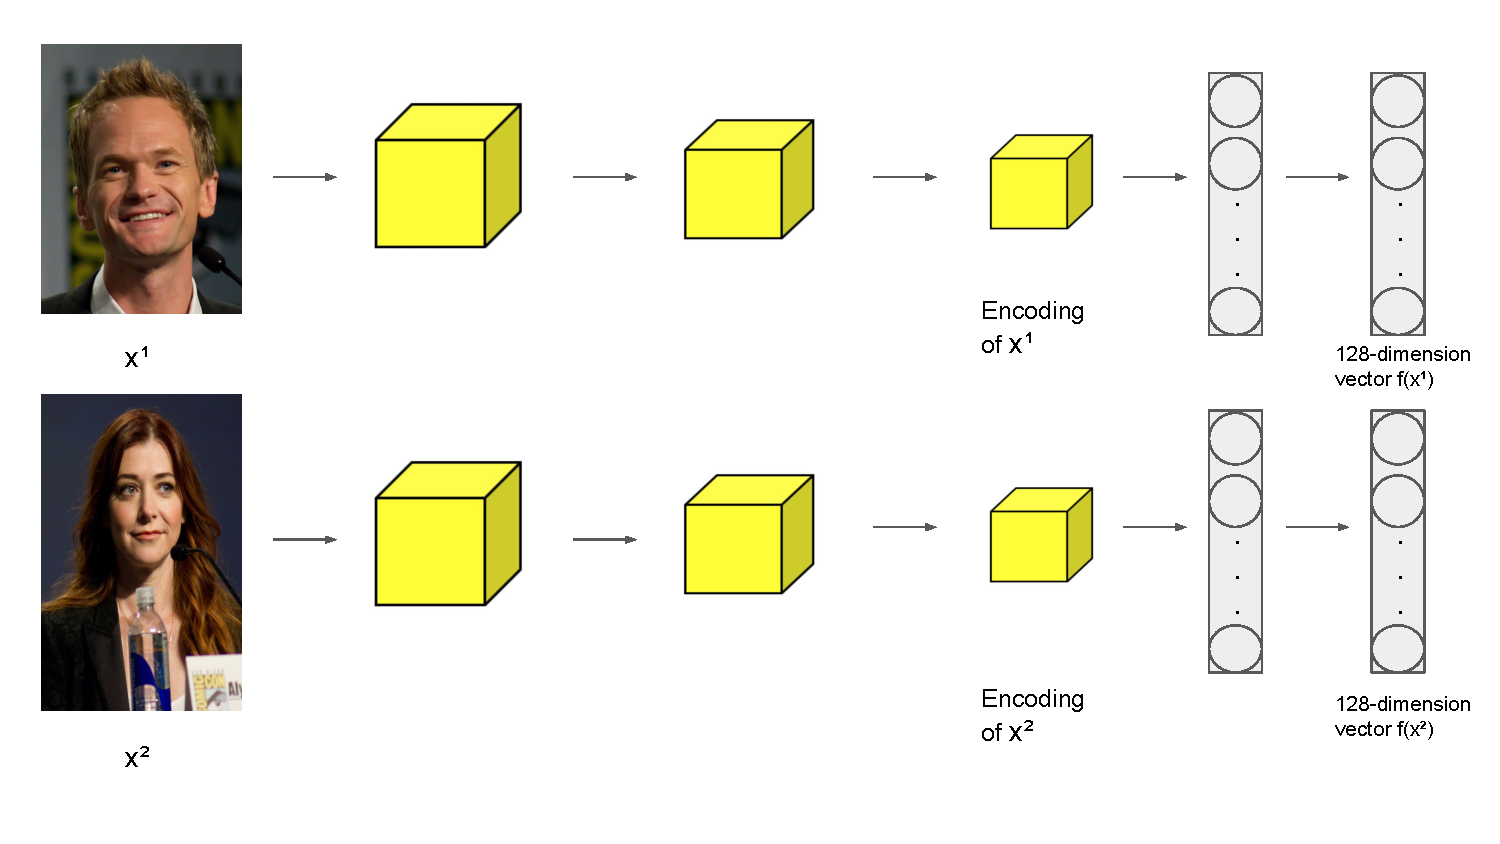
\includegraphics[scale=0.5]{siameseNetwork.pdf}
    \caption{Example of Siamese network}
    \label{fig:siameseNet}
\end{figure}

We conclude if two pictures were the same person by this function:

\begin{center}
    $
    \delta(x_1,x_2) = 
    \begin{cases}
        min ||f(x_1)- f(x_2)|| & \text{two person are the same} \\
        max ||f(x_1)- f(x_2)|| & \text{two person are different} \\
    \end{cases}
    $
\end{center}

\subsection{\acrlong{cnn}}
\paragraph{}

\acrfull{cnn} is a Deep Learning neural network that can take structured arrays of data like images, analyzing properties, aspects from the input images to differentiate one from the other. The name \acrlong{cnn} shows that it employs the mathematical convolution operation. We can stack up layers inside it for our purpose. For example: with three layers, the network can recognize handwriting; with 25 layers, the network can recognize human faces. We can add more layers for extracting and recognizing more features.

\begin{figure}[H]
    \centering
    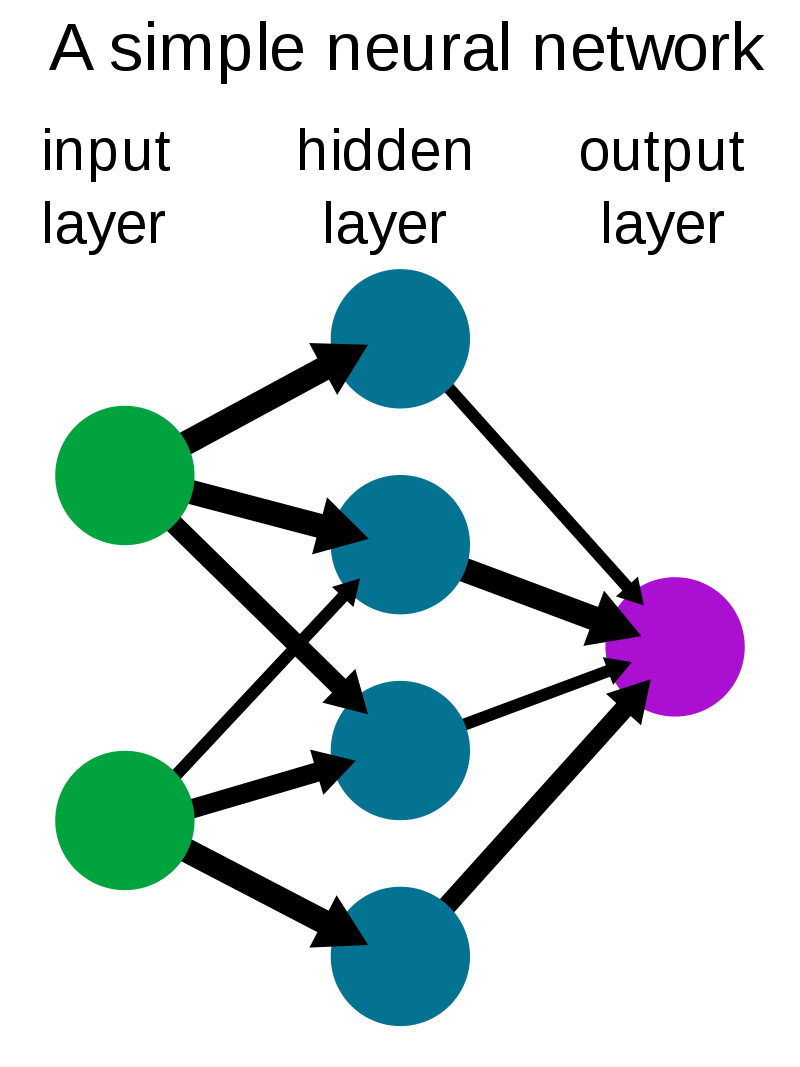
\includegraphics[width=0.3\textwidth]{Neural_network.png}
    \caption{Simple neural network}
    \caption*{\textit{source: Wikipedia}}
    \label{fig:simpleCNN}
\end{figure}

The \acrshort{cnn} was typically built by three main layers:

\begin{itemize}
    \item \textbf{Input layer}: takes input images then fits them into the network.
    \item \textbf{Hidden layers}: contains layers that perform a specific task.
    \item \textbf{Output layer}: decide which one belongs to which class.
\end{itemize}

We can control how many layers are inside hidden layers, but there are three main layers in it:
\begin{itemize}
    \item {Convolutional layer}: This layer extracts features from the image by taking the dot product between the image and a set of a learnable parameter known as the kernel. The kernel is smaller than the image but more in depth. 
    
    \begin{figure}[H]
        \centering
        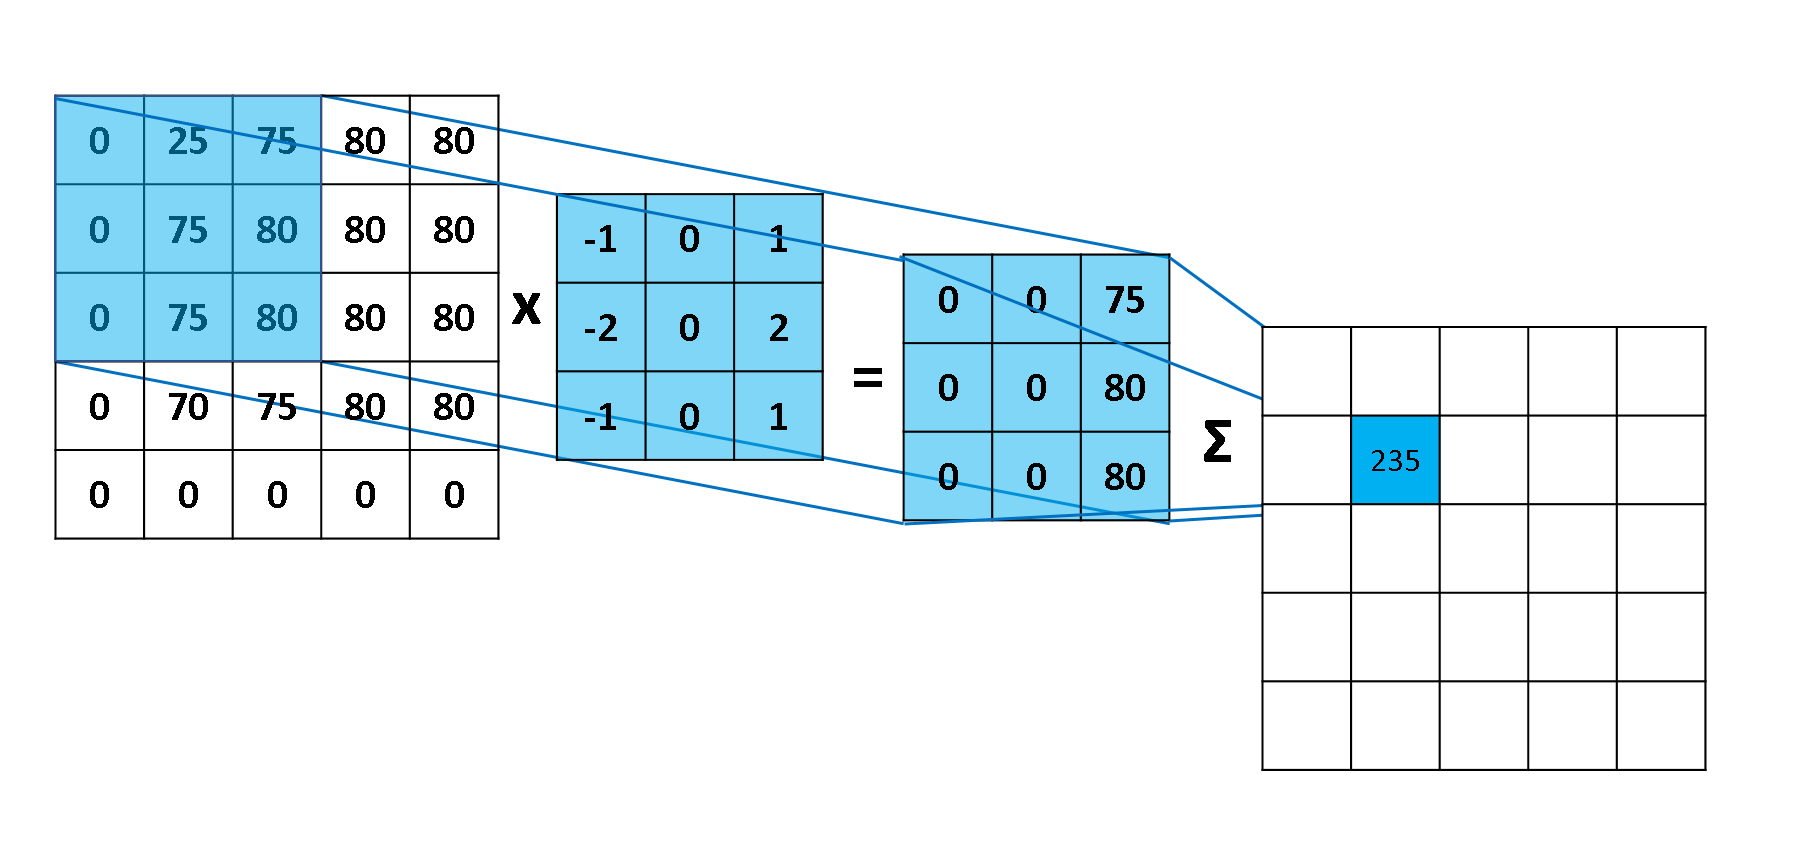
\includegraphics[width=0.7\textwidth]{convolutional_layer.png}
        \caption{Convolutional layer}
    \end{figure}
    During the forward pass, the kernel slides across the image, creating a two-dimensional image representation. The sliding size of the kernel is called \textbf{stride}. The bigger stride, the faster the kernel slide across the image.
    
    It can be seen that the feature map should be smaller if the kernel size is bigger. To avoid reducing feature map size after every convolutional layer, we have \textbf{padding} with value zero for having the image and feature map in the same size. The model contains many feature maps for extracting features from the input. It includes a stack of feature maps with different kernel values to extract clear features.
    
    \item {Activation layer}: The Activation layer is put at the end or between the \acrlong{cnn}. It helps to calculate the argument for the next layer. We have different activation functions like Rectified Linear Unit (ReLU), sigmoid, and softmax. Commonly ReLU is used after the Convolutional layer, sigmoid and softmax are used at the classification output layer.
    
    \begin{figure}[H]
        \centering
        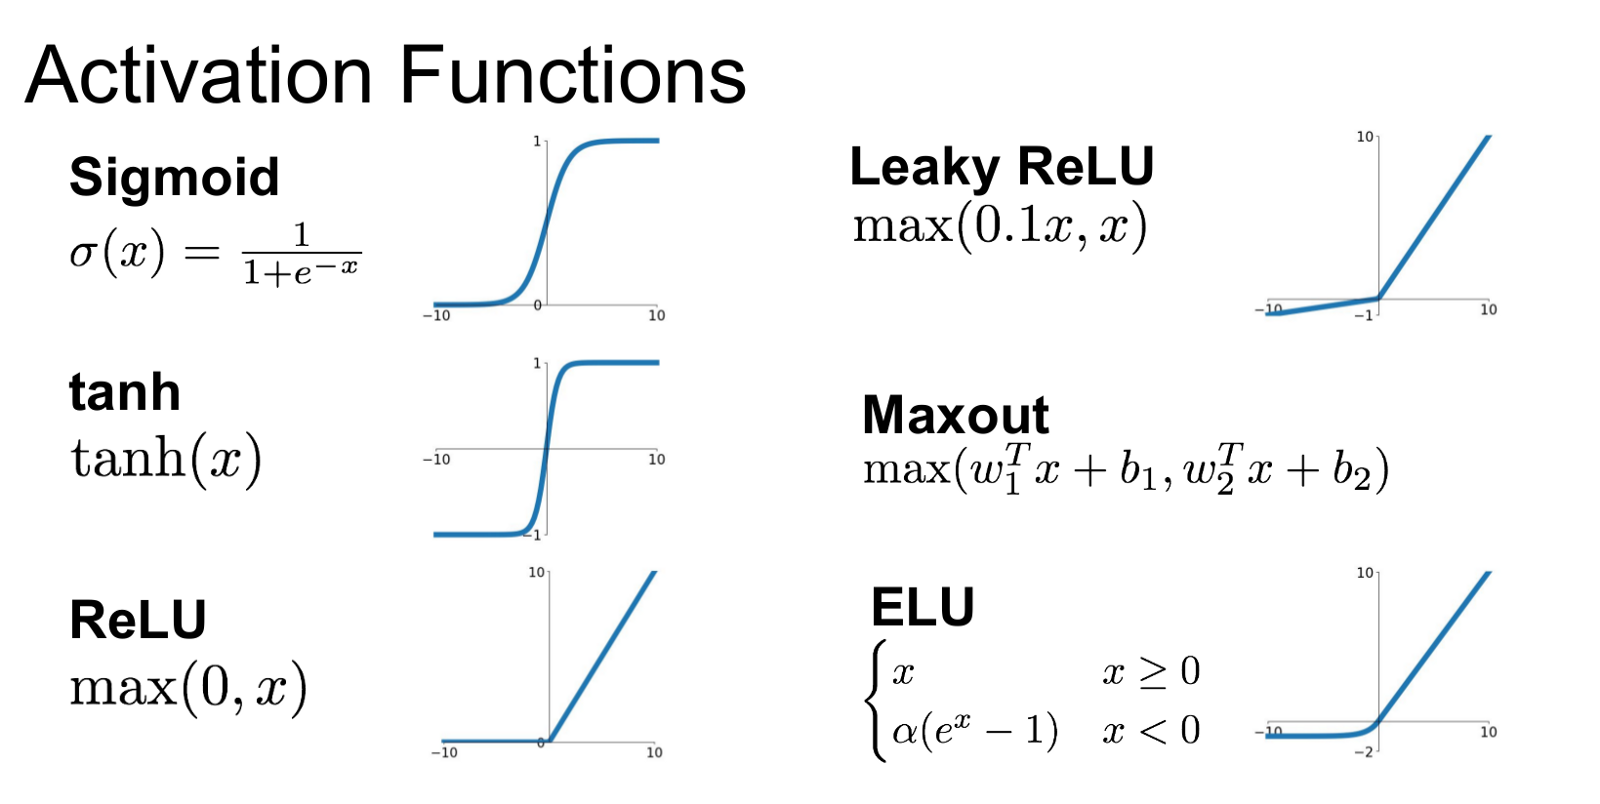
\includegraphics[scale=0.3]{activationLayer.png}
        \caption{Activation functions}
    \end{figure}
    
    \item {Pooling layer}: The pooling layer replaces the output of the network at some locations by deriving summary statistics of nearby outputs. It reduces the number of parameters and computations in the network, spatial size of the network to control overfitting. 
    
    There are two operations in this layer:
    
    \begin{itemize}
        \item Max Pooing: like its name states, it takes the max value from a pool.
        \begin{figure}[H]
            \centering
            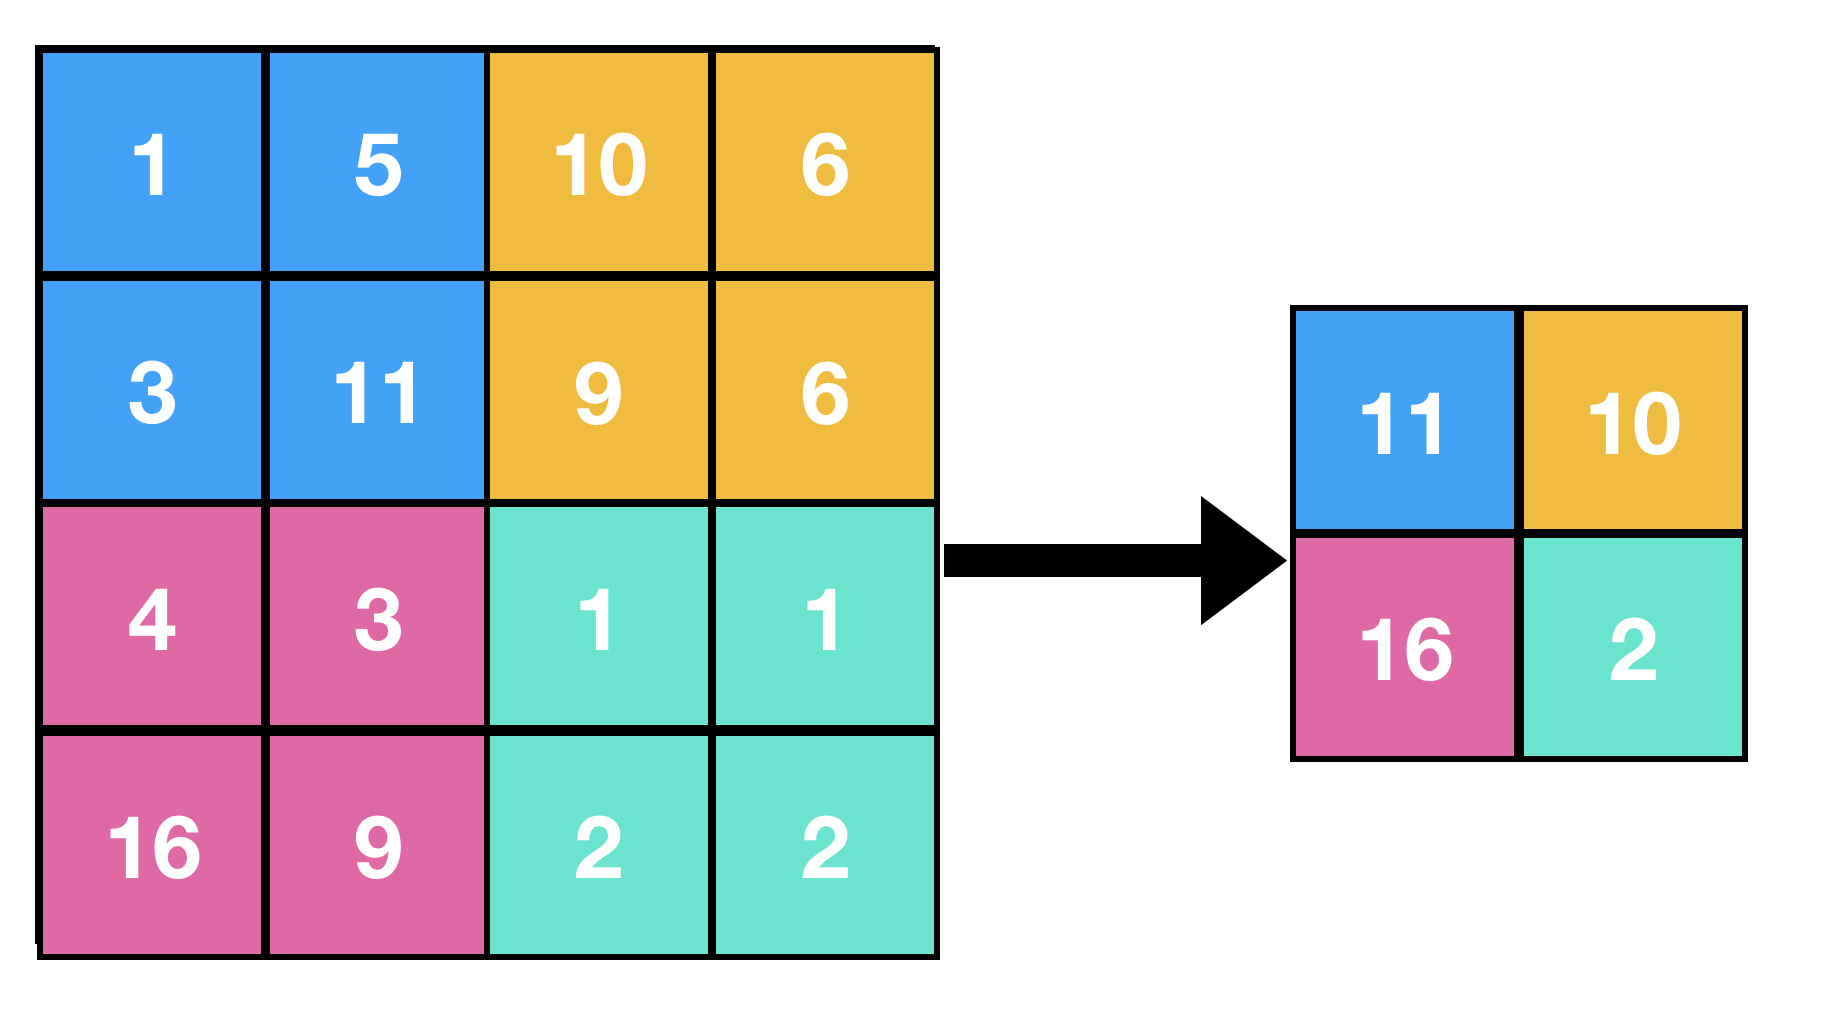
\includegraphics[width=0.3\textwidth]{Maxpooling.png}
        \end{figure}
        
        \item Average Pooing: it takes the average values from all value from a pool.
        \begin{figure}[H]
            \centering
            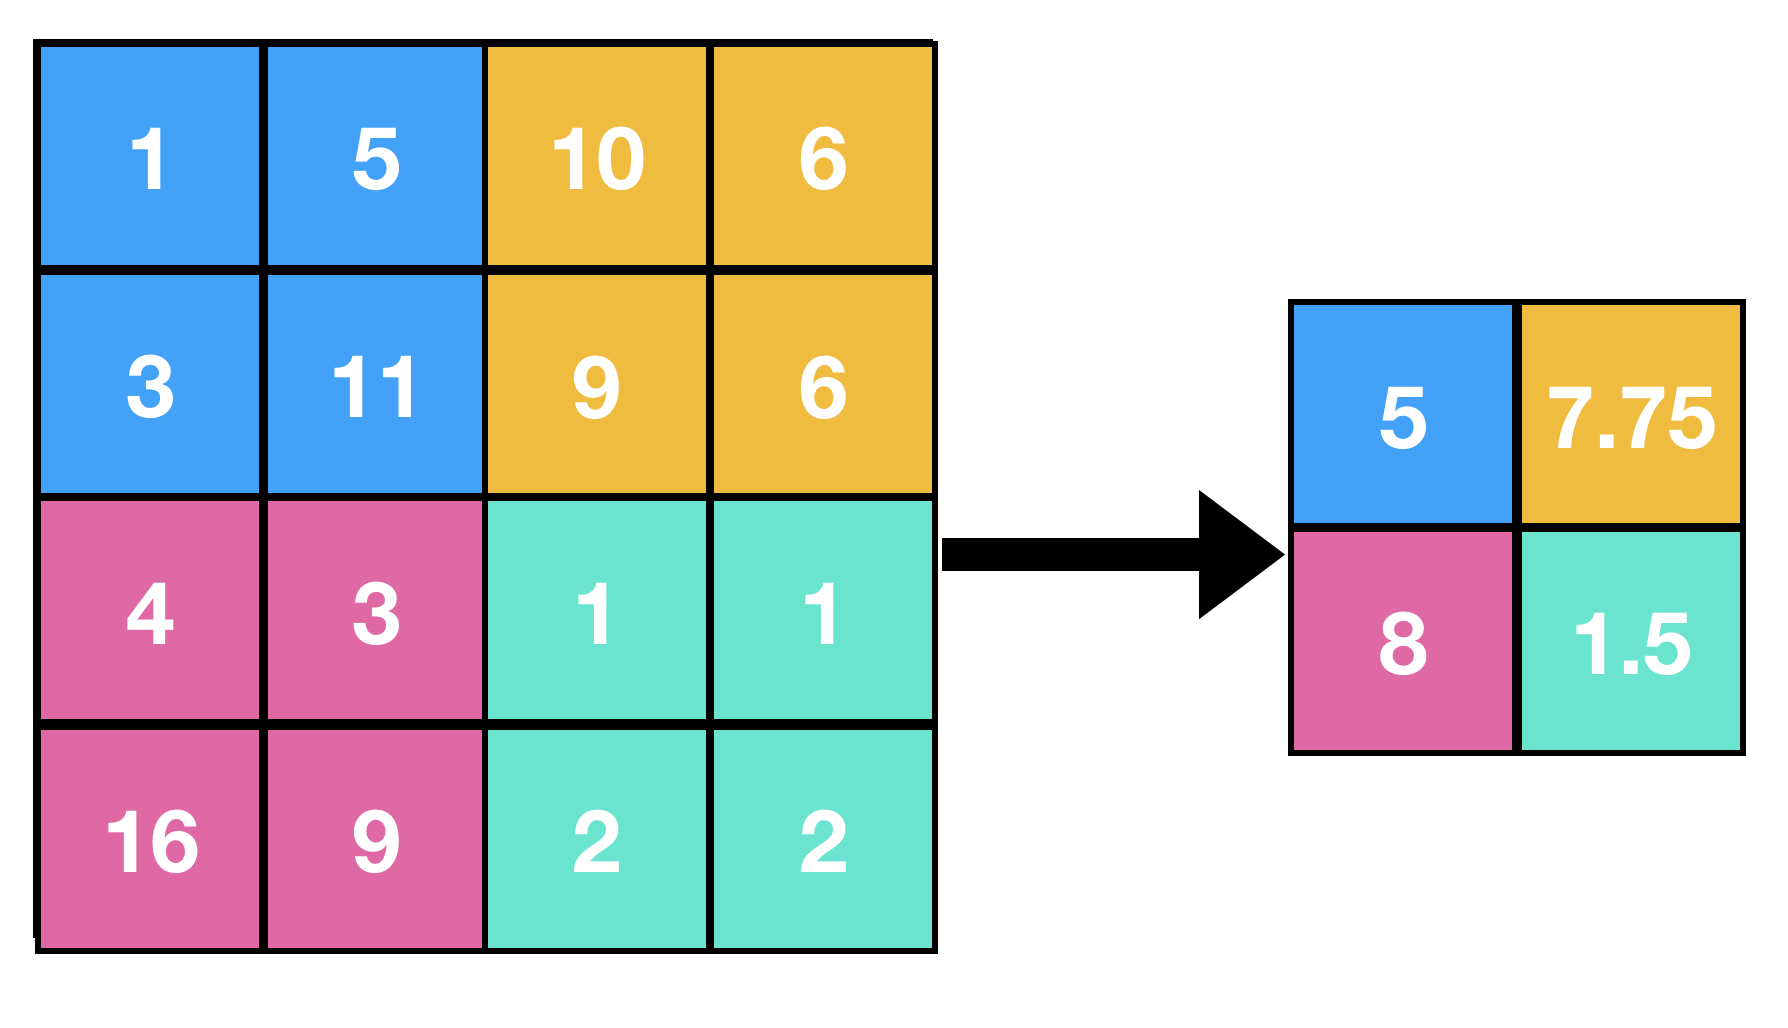
\includegraphics[width=0.3\textwidth]{Avgpooling.png}
        \end{figure}
    \end{itemize}
    
    \item {Fully Connected layer}: Neurons in this layer have a complete connection with all neurons from the previous layers. It can be computed by matrix multiplication followed by a bias offset. Fully Connected layers compile data extracted from earlier layers to get the final output.

    \item {Dropout layer}: Randomly drop connection from the previous layer.
    
    \item {Batch Normalization}: Normalize and scale data after each activation.
    
\end{itemize}

The combination of all these above layers is the basic concept of the \acrshort{cnn} model, as in figure \ref{fig:cnnDesign}.

\begin{figure}[H]
    \centering
    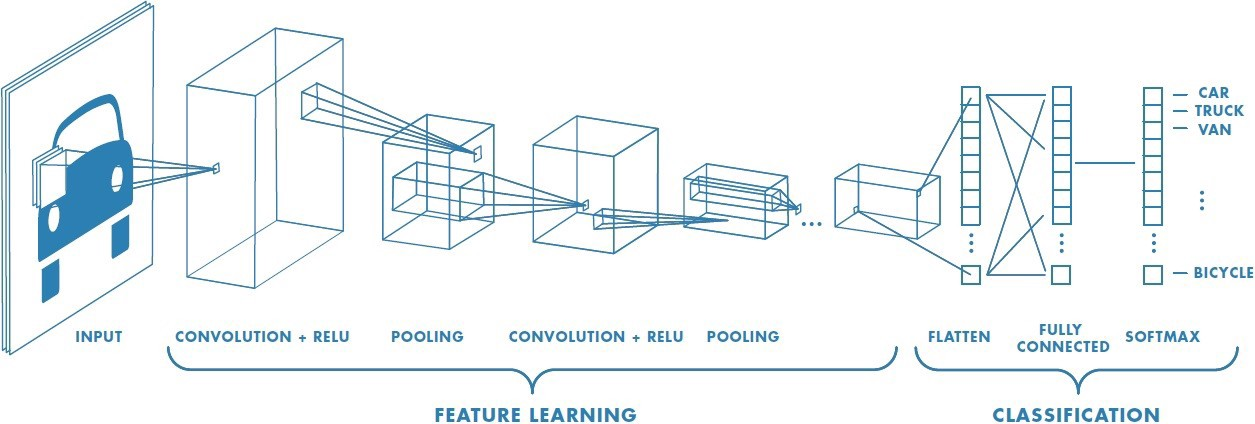
\includegraphics[scale=0.3]{convolutionalNetwork.jpeg}
    \caption{Basic concept of \acrshort{cnn}.}
    \label{fig:cnnDesign}
\end{figure}

\subsection{Flask}
\paragraph{}
Flask is a micro web framework written in Python. Flask takes advantage of the simplicity of Python, which makes it easy to build a primary application to backend APIs. It is classified as a micro-framework because it does not require any libraries. 

It is also called a \acrlong{wsgi} (\acrshort{wsgi}) framework. Flask gives us many choices when developing web applications and provides the necessary tools to build and deploy a web. Here are some of the merits of using Flask: 

\begin{enumerate}
    \item \textbf{Easy to use}: Flask framework is easy to understand. The simplicity in the framework helps us to navigate around and create applications easily.
    \item \textbf{Very flexible}: Most of the components of Flask can be altered. It allows users to customize the website.
    \item \textbf{Testing}: It allows unit testing through its integrated support, built-in development server, fast debugger, and RESTful request dispatching.
\end{enumerate}

\clearpage
\section{Methods}

\subsection{Building a Face recognition system}

\subsubsection{FaceNet}
\paragraph{}
In 2015, Florian Schroff et al.\cite{DBLP:journals/corr/SchroffKP15} introduced FaceNet. It transforms the face image into 128 dimensions Euclidean space, similar to word embedding. Once the FaceNet model having been trained with triplet loss for different classes of faces to capture the similarities and differences between them, the 128-dimensional embedding returned by the FaceNet model can be used to clusters faces effectively. It is the backbone of many open-source face recognition models like OpenFace\footnote{\url{https://cmusatyalab.github.io/openface/}}, facenet\footnote{\url{https://github.com/davidsandberg/facenet}}, etc.

\begin{figure}[H]
    \centering
    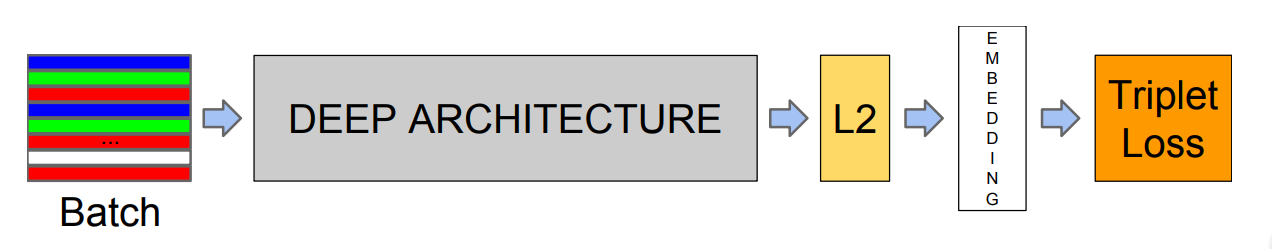
\includegraphics[scale=0.5]{facenetArchitecture.png}
    \caption{FaceNet Architecture}
\end{figure}

FaceNet has solved two problems in face recognition algorithm before it:
\begin{enumerate}
    \item Apply a \acrshort{cnn} and use 128-dimensional data to not need a bottleneck layer for reducing data dimensionally.
    \item Loss function can learn the similarity between two pictures in the same class or distinguish two pictures in different classes simultaneously.
\end{enumerate}

This model outputs an embedding of image $f(x)$ with $L_2$ normalization on it. After that, these embeddings pass into a loss function to make the squared distance between two images is small when two images belong to the same identity, whereas the squared distance will be significant. This loss function is called \textbf{Triplet loss}. 

\subsubsection{Triplet loss}
\label{tripletLoss}
\paragraph{}
The encoding of the \acrlong{cnn} helps us encode the picture into a 128 dimensional vector $f(x)$ called embedding. It is normalized such that:

\begin{center}
    $||f(x)||^2_2=1$
\end{center}

To implement Triplet loss, we need to take three pictures, including: anchor picture ($x^a_i$), positive picture ($x^p_i$) which is a picture of the same person), negative picture ($x^n_i$) which is from the different person, to satisfy that:

\begin{center}
    $||f(x^a_i) - f(x^p_i)||^2_2 + \alpha < ||f(x^a_i) - f(x^n_i)||^2_2$
\end{center}

$\alpha$ is an enforced margin to differentiate between positive and negative pairs. So that the loss function can be defined:

\begin{center}
    $\mathcal{L}(x^a,x^p,x^n)=\Sigma^n_i[|f(x^a_i) - f(x^p_i)||^2_2 - ||f(x^a_i) - f(x^n_i)||^2_2 + \alpha]$
\end{center}

\begin{figure}[H]
    \centering
    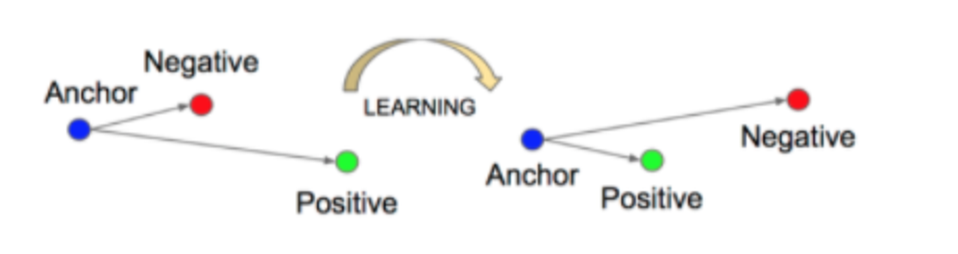
\includegraphics[scale=0.5]{tripletLoss.pdf}
    \caption{Triplet loss learning}
\end{figure}

If the above function can easily be satisfied by choosing close triplets, it would not help the training. So choosing triplets that violate that function is essential.

\subsubsection{Triplet images input selection}
\paragraph{}
If the chosen triplets were easy to distinguish, the learning images would not make any sense. We need to choose hard triplets to make the model harder to learn and help the model discriminate effectively between faces.

\begin{figure}
    \centering
    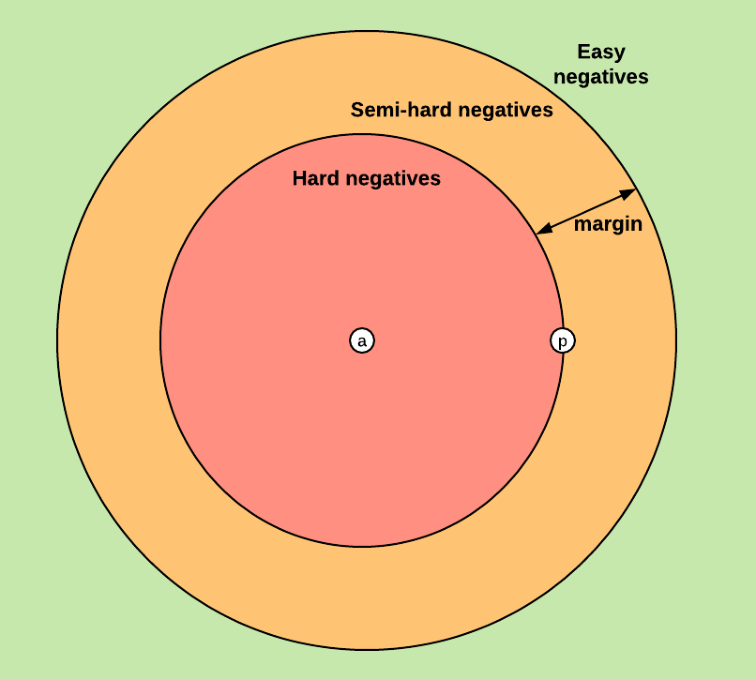
\includegraphics[scale=0.5]{tripletSelection.pdf}
    \caption{Chossing hard triplets}
\end{figure}

This mean that for a given $x^a_i$, we need to choose 2 pairs of anchor-positive and anchor-negative to please:
\begin{enumerate}
    \item Hard positive: $\argmax(|f(x^a_i) - f(x^p_i)||^2_2)$
    \item Hard negative: $\argmin(||f(x^a_i) - f(x^n_i)||^2_2)$
\end{enumerate}

Computing \textbf{Hard positive} and \textbf{Hard negative} can do on the previous checkpoint or do it on every mini-batch to minimize computationally expense when generating the whole training data set. Choosing triplets on purpose can make the model giving the result more accurate. 

\subsubsection{Experimental with pre-trained FaceNet model}
\paragraph{}
Based on \hyperref[sec:siamese]{Siamese neural network}, we will choose a based network and drop out the output layer. VGG16 is one of the most powerful networks in the classification topic. It contains multi-layers of Convolutional, Pooling, and Fully Connected layers. The input runs through two convolutional layers with 64 filter channels of 3*3 kernel with the same padding from the input. Following a Max Pool layer of stride 2*2, two layers have convolution layers of 256 filter channels with filter size 3*3. Then there is a Max Pooling layer of stride 2*2, following by two convolution layers of filter size 3*3 and 256 filter channels. There are two sets of 3 convolution layers and a max pool layer, and each has 512 filters of 3*3 sizes with the same padding. After all, the data is passed through three fully connected layers.

\begin{figure}[H]
    \centering
    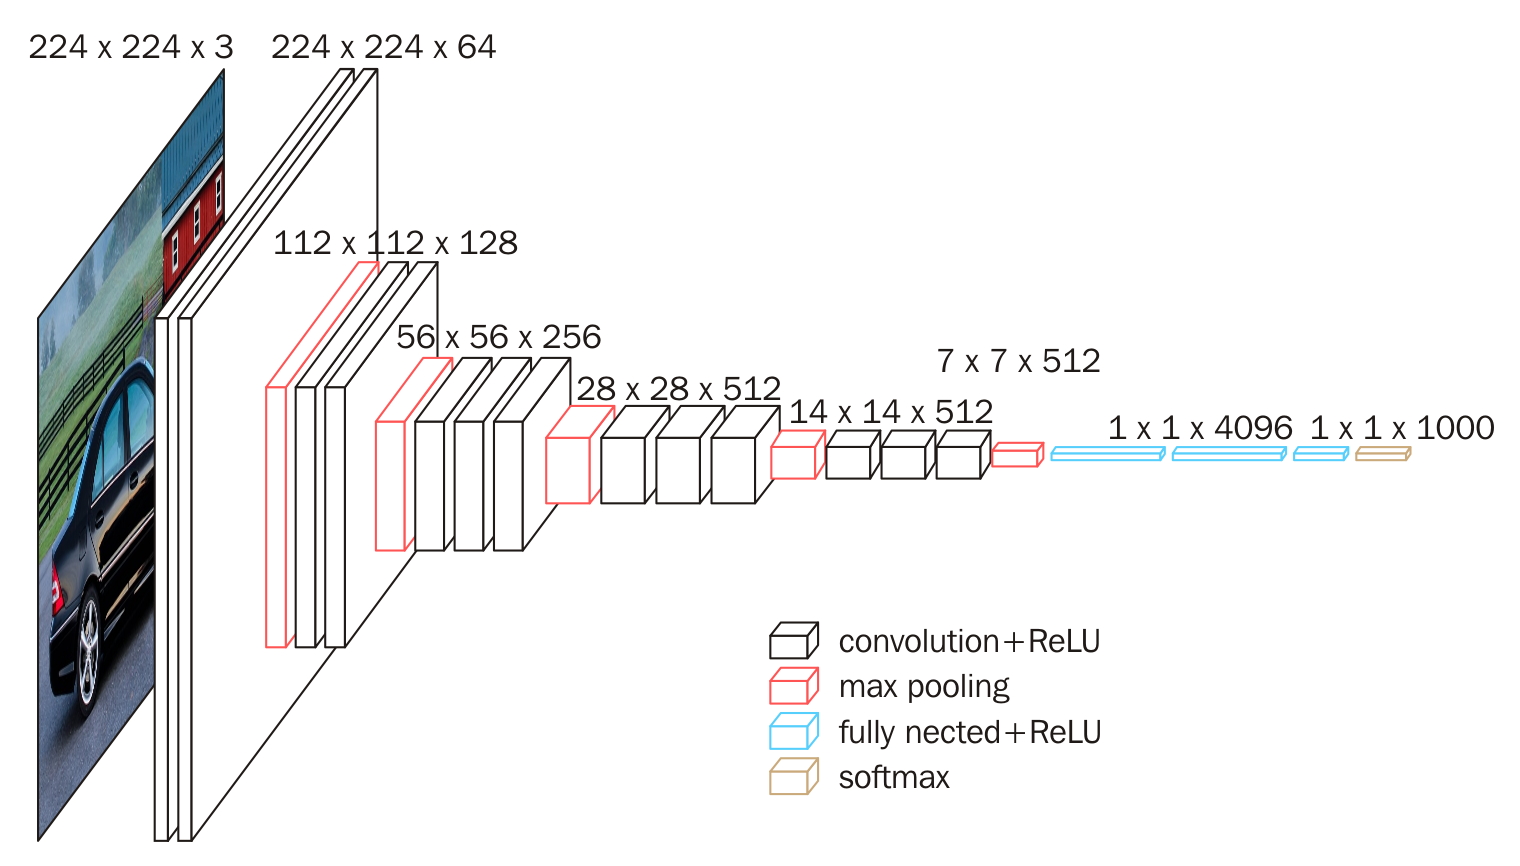
\includegraphics[width=0.8\textwidth]{VGG16.png}
    \caption{Architecture of VGG16 network.}
    \caption*{\textit{source: towardsdatascience.com}}
    \label{fig:VGG16}
\end{figure}

After getting the base network, we add the Triplet loss function to determine the input belongs to which class. To save training time, we are using the weights from OpenFace\footnote{\url{https://cmusatyalab.github.io/openface/}} model. We will train the model with VN-celeb dataset, published by Sun* AI team, to use this with Vietnamese people.

\subsubsection{Making the recognition system}
\paragraph{}
We are using the trained model, OpenCV, and MTCNN to create the system. To avoid using an image to spoof the system, we are setting up two lights from behind the camera. If someone came with a picture, the system would not detect it.

First, we are connecting the camera to the server. The server has a job that captures every frame that contains the human face with the help of OpenCV. The model implemented on the server creates embedding vectors for every registered face in the database. Moreover, these vectors are stored only in the running state and deleted after the system stops to avoid outside access.

After that, the system creates an embedding vector for the current face that shows at the camera, which is detected using Haar Cascade. Compare with a recent detecting model like dlib\footnote{\url{https://github.com/davisking/dlib}}, \acrshort{mtcnn}\cite{Zhang_2016}, OpenCV \acrshort{dnn} Face Detector, Haar Cascade shows some outdated and worst result in detecting faces in a picture that has many faces in that or large picture size. Besides, it also depends much on lighting, face rotation, and the quality of the image. But during the recognition, there is only one person at the camera at that time. And faces in the database with face in the camera are equal in lighting and quality. So using the Haar Cascade is the best option for us at the detecting time.

\begin{figure}[H]
    \centering
    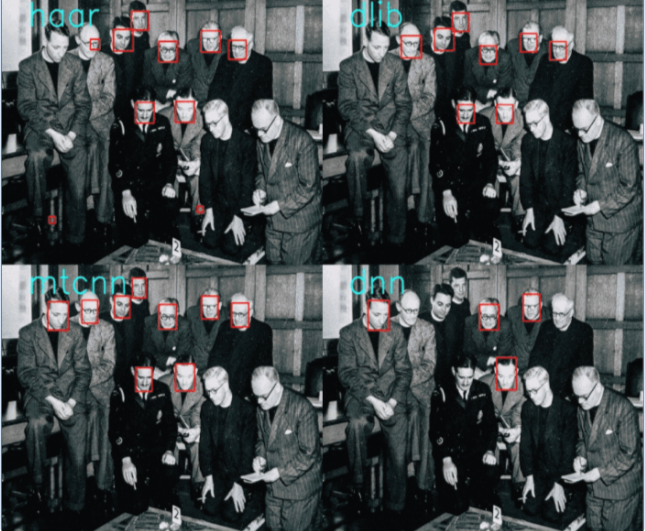
\includegraphics[scale=0.6]{comparisonHaar.png}
    \caption{Comparison along with face detection model}
    \caption*{\textit{source: Vardan Agarwal - towardsdatascience.com}}
\end{figure}

Since we got vectors from the database and the vector from the camera, the system will calculate the Euclidean distance with these vectors to find the smallest compare with the threshold we choose.

After the recognition is finished, the liveness test will continue. The liveness test is for avoiding people using a printed image to trick the system. We are using \acrshort{mtcnn} to extract key points from the face. It will store the default key points of the face. \acrshort{mtcnn} detector will track the key points. When it satisfies the math function of calculating the distance of eyes and nose, the system will request the \acrlong{ccu}.

\begin{figure}[H]
    \centering
    \includegraphics{dataflow.png}
    \caption{Recognition system data flow}
\end{figure}

\subsection{\acrshort{iot} devices setup and API connection}
\subsubsection{\acrshort{iot} devices setup}
\paragraph{}
\acrshort{iot} is one of the buzzwords in the technology industry in the past years, stands for \acrlong{iot}. \acrshort{iot} means all of the things that are connected to the Internet and can be controlled remotely. According to Wikipedia\footnote{\url{https://en.wikipedia.org/wiki/Internet_of_things}}: 
"..the network of physical objects - devices, vehicles, buildings, and other items - embedded with electronics, software, sensors, and network connectivity that enables these objects to collect and exchange data."

The main factor in the upwards trend in \acrshort{iot} systems is DIY (do it yourself) electronic platforms like Raspberry Pi and Arduino. Raspberry Pi (figure~\ref{fig:raspi}) has many advantages: small, inexpensive, easy to use, etc. And after all, it allows us to connect various accessories via a 40-pins \acrshort{gpio} connection built-in on board.

\begin{figure}[H]
    \centering
    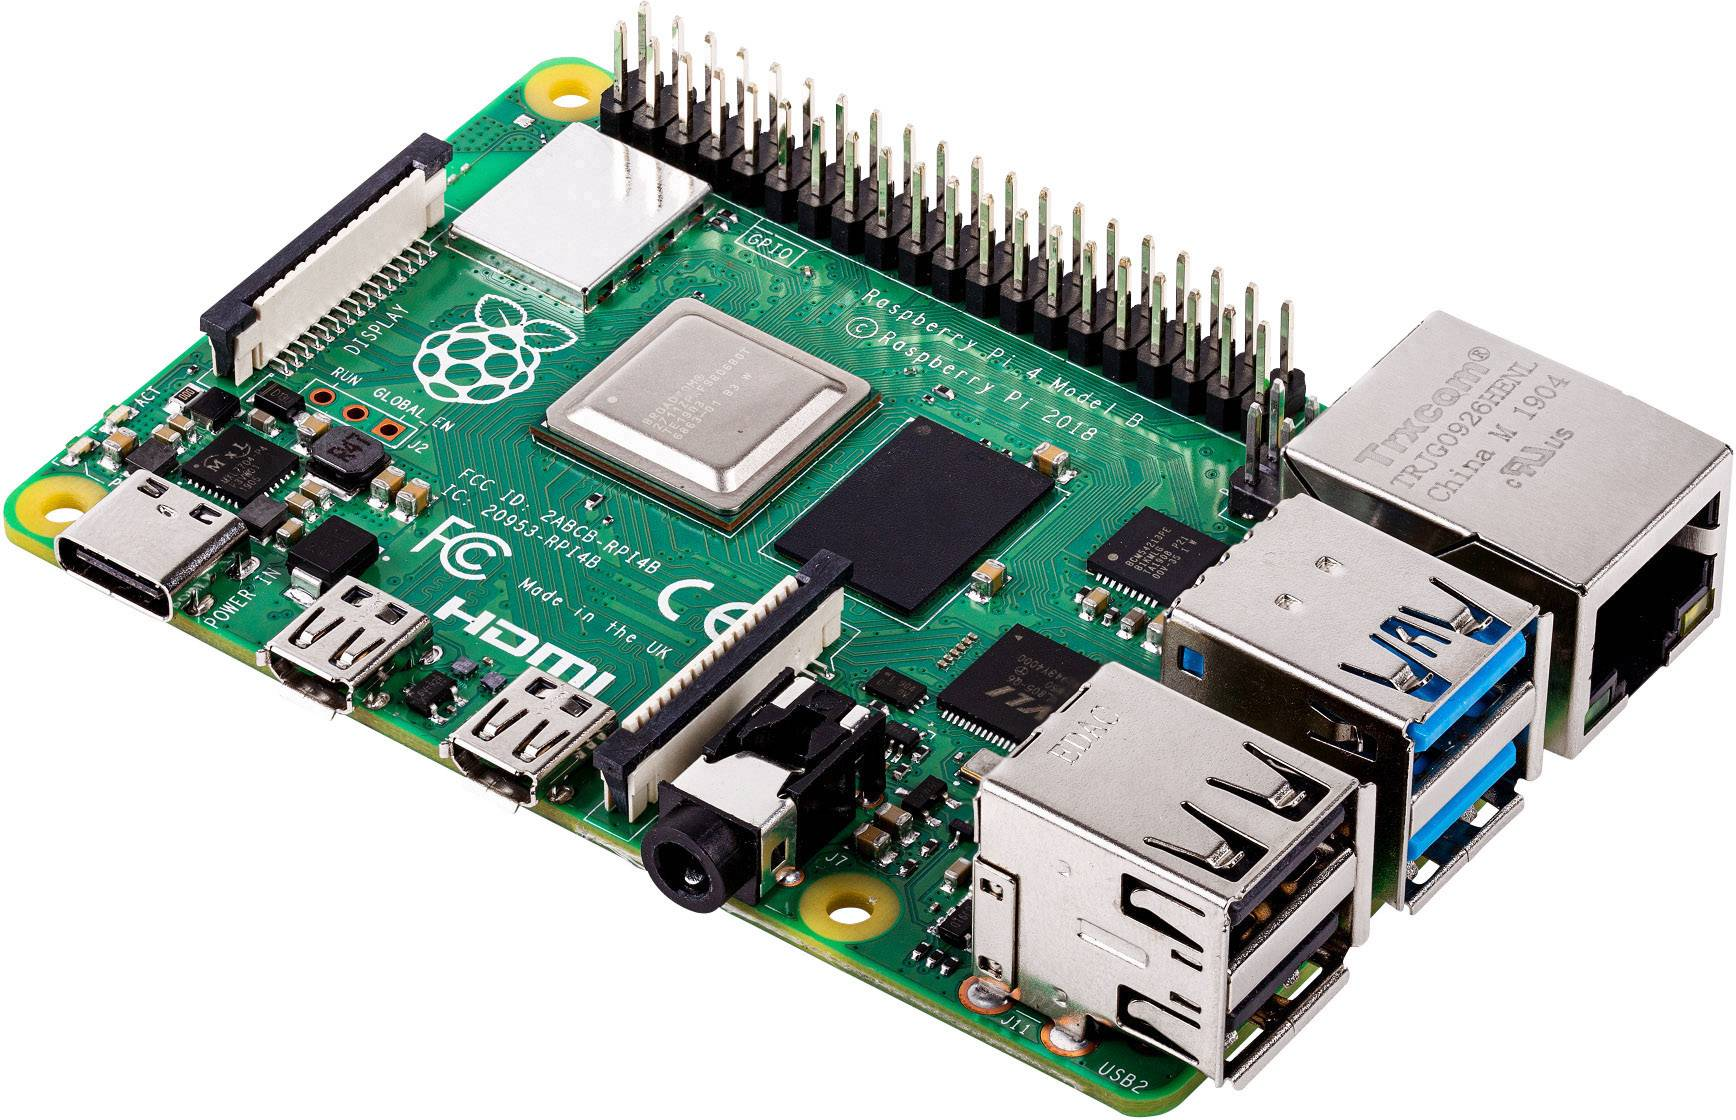
\includegraphics[scale=0.15]{raspPi.png}
    \caption{Raspberry Pi board}
    \label{fig:raspi}
\end{figure}

To interact with all \acrshort{iot} devices, we use Raspberry Pi version 4 with a specification in table~\ref{tab:raspiSpecs} as a \acrshort{ccu}(\acrlong{ccu}).  

\begin{table}[H]
    \centering
    \caption{\acrlong{ccu} specification}
    \begin{tabular}{|c|c|}
        \hline
        OS & Raspberry Pi OS \\
        \hline
        Kernel version & 5.10\\
        \hline
        CPU & Quad-core Cortex-A72 (ARM v8) 64-bit Soc \\
        \hline
        RAM & 4GB\\
        \hline
    \end{tabular}
    \label{tab:raspiSpecs}
\end{table}

Since the limitation of the voltage output of the \acrshort{ccu} device, we are controlling one electric door lock and two light bulbs. The diagram of connecting electric door lock is in figure~\ref{fig:doorLockDiag}

\begin{figure}[H]
    \centering
    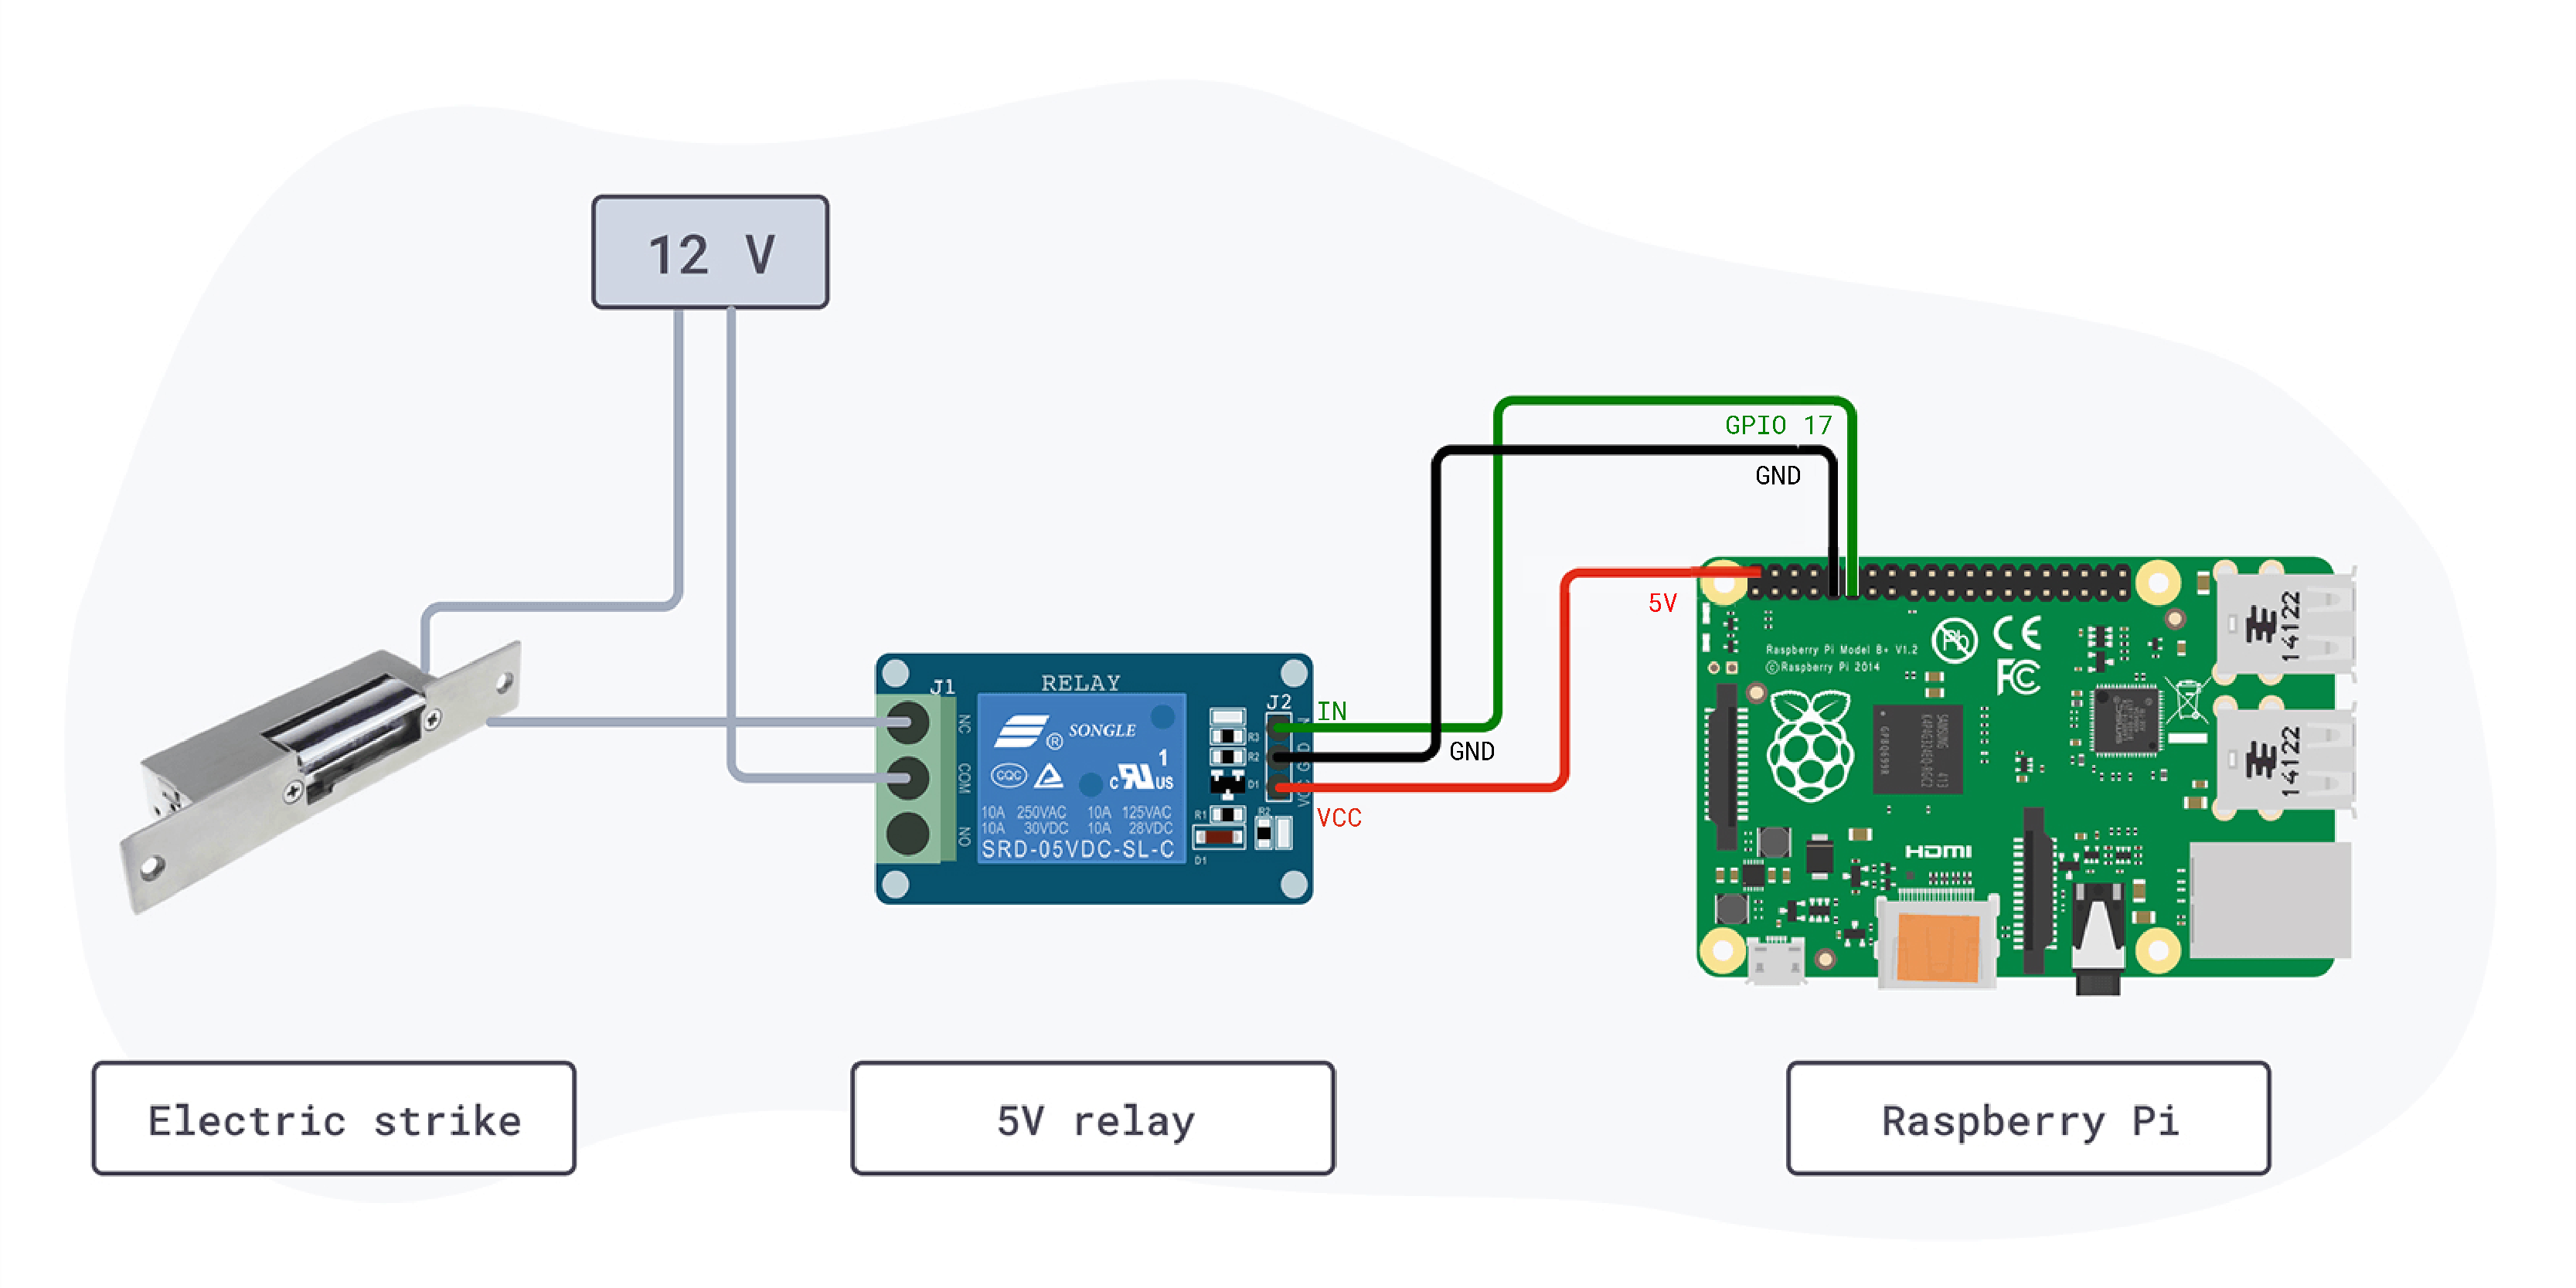
\includegraphics[scale=0.2]{piSetup.pdf}
    \caption{Electric door lock connection diagram}
    \label{fig:doorLockDiag}
\end{figure}

We are using a 12V DC lock. So we connect the lock with a 12V external power, which is three 3.7V 18650 batteries. We are using a 5V relay for controlling the switch with code. The connection between \acrshort{ccu} and relay: connect \textbf{5V \acrshort{gpio} pin} to \textbf{VCC} for power to the relay, \textbf{GND pin} to \textbf{GND} for ground, \textbf{\acrshort{gpio} 17} to \textbf{IN} for controlling.

The central part of controlling the lock is connecting the lock and external power to the relay. Here we connect the lock to \textbf{\acrshort{nc}} (\acrlong{nc}); External power to \textbf{\acrshort{com}} (\acrlong{com}). The \acrshort{com} connection is the moving part of the relay. We set the initial state of the INPUT from \acrshort{ccu} as \textbf{GPIO.low}, High/Low switch on the relay to \textbf{High}. This setup works from the initial setup before; If the input from \acrshort{ccu} is low, then the lock does not have any power equal to lock state; else, if the input is high, then the lock has power equal to unlock state. We are setting the lock state to \textbf{GPIO.low}, unlock state to \textbf{GPIO.high}.

For light bulbs, the setup is much simpler:

\begin{figure}[H]
    \centering
    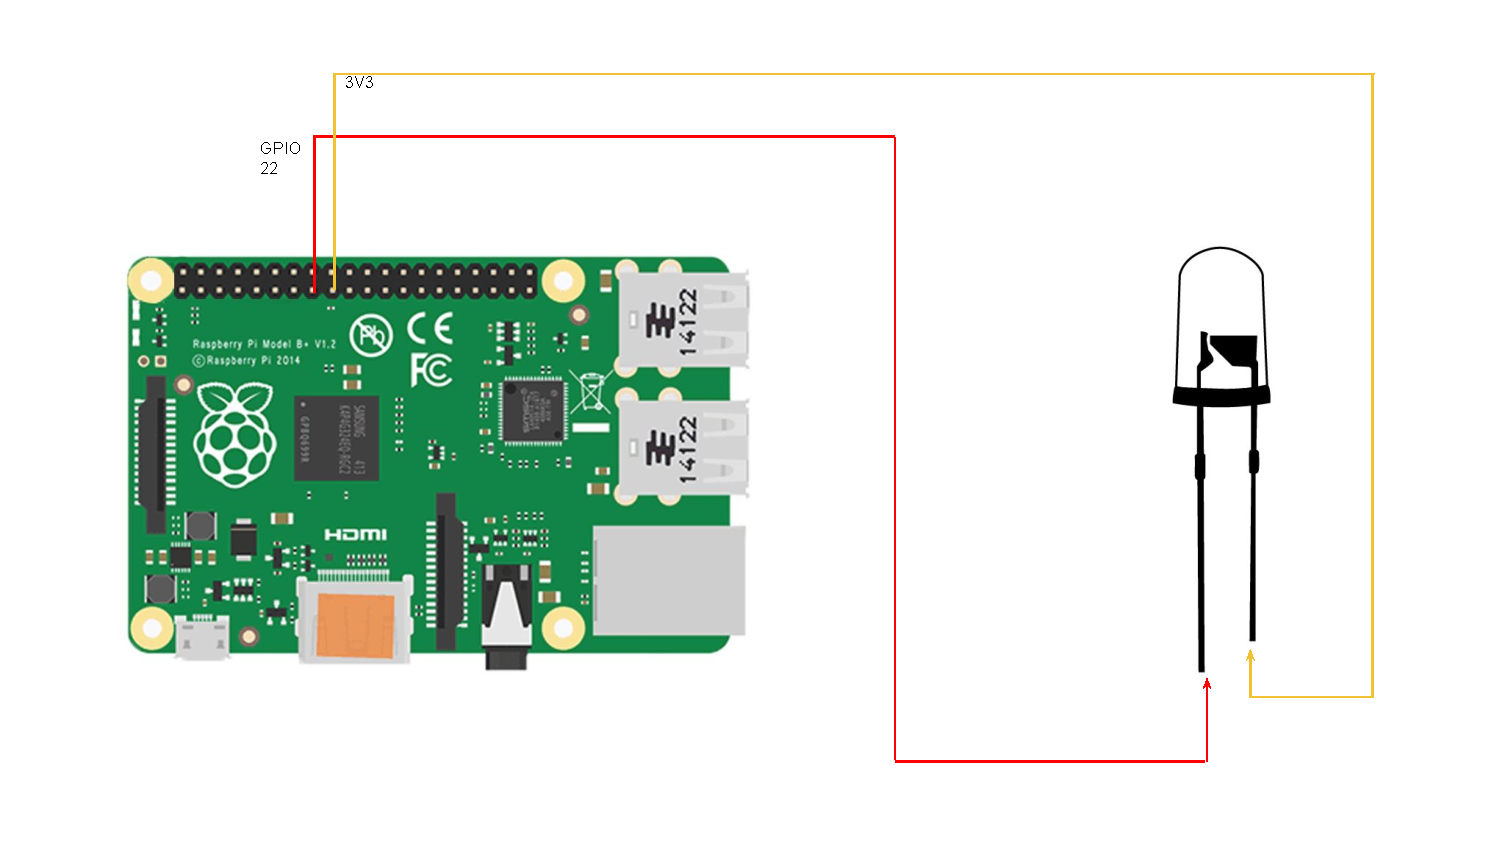
\includegraphics[scale=0.4]{lightSetup.pdf}
    \caption{Light bulbs connection diagram}
\end{figure}

We connect one pin to \textbf{GPIO 22} pin to control, the other to a \textbf{3V3} pin for power. We set automation for every unlock, and the light turns on for two minutes for a home scenario.

\subsubsection{Google Assistant \acrshort{sdk}}
\paragraph{}
The best way to set up a smart home with \acrshort{iot} devices is automation. Because of the limitation of our \acrshort{ccu}, adding Google Assistant \acrshort{sdk} to it will extend the ability to connect more smart devices using the Google Home network.

Google Developers team has clear documentations\footnote{\url{https://developers.google.com/assistant/sdk/guides/service/python#steps}} about how to implement it on a Raspberry Pi using Python.


\subsubsection{\acrshort{api} connection}
\paragraph{}
To connect a server for Face recognition to \acrlong{ccu}, we create an \acrfull{api} using Flask to link these two components.

\begin{figure}[H]
    \centering
    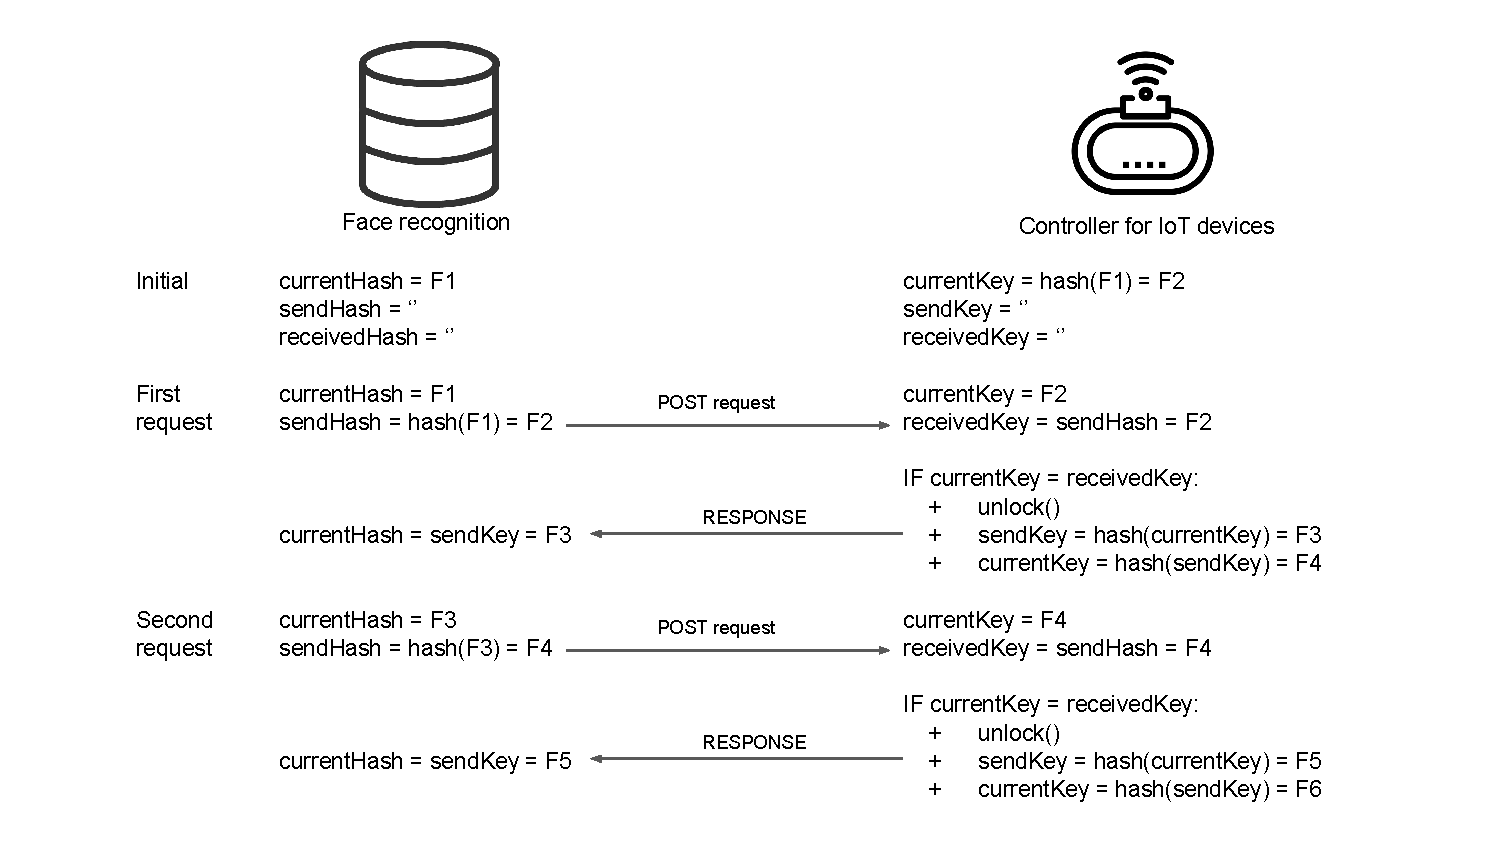
\includegraphics[scale=0.7]{apiDiagram.pdf}
    \caption{API connection flow}
    \label{fig:apiDiag}
\end{figure}

We are applying a blockchain-like method on \acrshort{api} for security. Both server and \acrshort{ccu} has two different initial private key. For example, the initial private key on the server is F1, so the initial of \acrshort{ccu} is SHA-256 encode of F1. After every request, a private key that store on both side change, as shown in figure~\ref{fig:apiDiag}. If someone can hack to the connection, they neither can trace back to the first private key nor find out the encoding algorithm.

Latency in this system is also a problem to be a suitable replacement in real life since they share the same local network, the system work in almost real-time.

